\documentclass{article}
\usepackage[T1]{fontenc}
\usepackage{lmodern}
\usepackage{graphicx}
\usepackage{amsmath,amssymb}
\usepackage[a4paper,margin=2cm]{geometry}
\usepackage[absolute,overlay]{textpos}
\setlength{\TPHorizModule}{1mm}
\setlength{\TPVertModule}{1mm}
\usepackage[indonesian]{babel}
\usepackage{hyperref}
\setlength{\emergencystretch}{2em}
% unit: Halaman 2

\begin{document}

% === Halaman 2 (llm) ===

\begin{itemize}
    \item Misalkan Alice dan Bob saling berkomunikasi dengan berkirim pesan:
    \begin{itemize}
        \item via surat menyurat,
        \item via telepon
        \item via email
        \item via SMS
        \item dll
    \end{itemize}
    menggunakan saluran komunikasi publik (pos, telepon, jaringan seluler, internet)
\end{itemize}
\vspace{10mm}

\vspace{74.25mm}

% deskripsi: Ilustrasi komunikasi antara Alice dan Bob dengan tanda panah yang menunjukkan pengiriman pesan dari Alice ke Bob.
% bbox normalisasi: [0.1850, 0.6300, 0.8300, 0.8800]
\begin{textblock*}{135.45mm}(38.85mm,187.11mm)
\noindent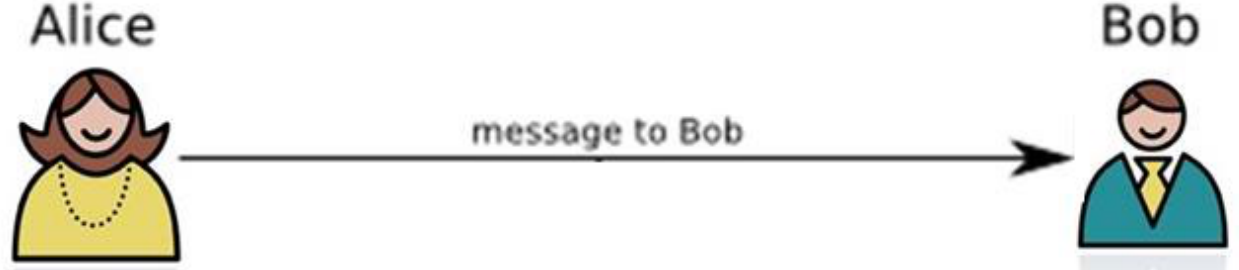
\includegraphics[width=135.45mm,height=74.25mm]{../../images/llm/page_002_img_01.png}%
\end{textblock*}

\end{document}
